\documentclass{crypto-exercise}
\usepackage{amsthm}
\author{Sven Laur}
\contributor[Initial solution]{Prastudy Fauzi}
\contributor[Fully reworked solution]{Sven Laur}
\editor{Sven Laur}
\tags{message authentication, authenticated encryption, non-malleability}

\newcommand{\ADVNMCPA}[2]{\ADV^{\mathsf{nm\text{-}cpa}}_{#1}{(#2)}}
\newcommand{\ADVMAC}[2]{\ADV^{\mathsf{mac}}_{#1}{(#2)}}

\newcommand{\ADVFNMCPA}[2]{\ADV^{\mathsf{nm\text{-}cpa}}_{#1}{(#2)}}
\newcommand{\CS}{\mathfrak{C}}

\newcommand{\AENC}{\mathsf{Auth\text{-}Enc}}
\newcommand{\ADEC}{\mathsf{Auth\text{-}Dec}}
\newcommand{\LENC}{\mathsf{LegitEnc}}
\newcommand{\GDEC}{\mathsf{GoodDec}}

\begin{document}


\begin{exercise}{Authenticate+Encrypt=NM-CPA}
Let $\CS=(\GEN,\ENC,\DEC)$ be a IND-CPA secure symmetric encryption scheme and let $h$ be a secure message authentication code with the appropriate message and key domains. Show that the paradigm first authenticate and then encrypt
\begin{align*}
      \begin{fblock}{\mathsf{Key\text{-}Gen}}
      & \SK\gets\GEN\\
      & k\gets\KSPACE\\
      & \RETURN (\SK,k)
      \end{fblock}
      &&
            \begin{aligned}
      \begin{fblock}{\AENC_{\SK,k}(m)}
      & t\gets h(m,k)\\
      & \RETURN \ENC_\SK(m,t)\\
      \end{fblock}\\
      \
      \end{aligned}
      \qquad\qquad
      \begin{aligned}       
      \begin{fblock}{\ADEC_{\SK,k}(c)}
      & (m,t)\gets\DEC_\SK(c)\\
      & \IF t\neq h(m,k)\ \THEN \RETURN \bot\\ 
      & \ELSE \RETURN m\\
      \end{fblock}\\
      \
      \end{aligned}
\end{align*}
assures non-malleability under chosen message attacks (NM-CPA security).

\end{exercise}
\begin{solution}

Let the encryption scheme $\CS$ be $(t_1, \varepsilon_1)$-IND-CPA secure and let $h$ be $(t_2, \varepsilon_2)$-secure message authentication code. Let us now consider the advantage of an adversary $\AD$ against NM-CPA games:
\begin{align*}
  \begin{game}{\GAME_0^\AD}
    &k\gets\KSPACE\\
    &\SK\gets\GEN\\
    &\MSPACE_0\gets\AD^{\AENC_{\SK,k}(\cdot)}(\PK)\\
    &m\gets\MSPACE_0, \overline{m}\gets{\MSPACE_0}\\
    &c\gets\ENC_{\SK,k}(m)\\
    &(\pi,\hat{c}_1,\ldots\hat{c}_n)\gets\AD^{\AENC_{\SK,k}(\cdot)}(c)\\
    &\IF c\in\set{\hat{c}_1,\ldots\hat{c}_n}\THEN \RETURN 0\\
    &\RETURN \pi(m,\ADEC_{\SK,k}(\hat{c}_1),\ldots)
  \end{game}
  \qquad\qquad
  \begin{game}{\GAME_1^\AD}
    &k\gets\KSPACE\\
    &\SK\gets\GEN\\
    &\MSPACE_0\gets\AD^{\AENC_{\SK,k}(\cdot)}(\PK)\\
    &m\gets\MSPACE_0,\overline{m}\gets{\MSPACE_0}\\
    &\pi,\overline{c}\gets\AENC_{\SK,k}(\overline{m})\\
    &(\pi,\hat{c}_1,\ldots\hat{c}_n)\gets\AD^{\AENC_{\SK,k}(\cdot)}(\overline{c})\\
    &\IF c\in\set{\hat{c}_1,\ldots\hat{c}_n}\THEN \RETURN 0\\
    &\RETURN \pi(m,\ADEC_{\SK,k}(\hat{c}_1),\ldots)\enspace.
  \end{game}
\end{align*}
Although the adversary $\AD$ does not make the explicit call to the decryption oracle, the form of the security game implies that $\AD$ is entitled to a singe decryption call, after which the predicate $\pi$ determines the output of the game. As a result, the following interaction diagram captures interactions in the game. 

\begin{center}
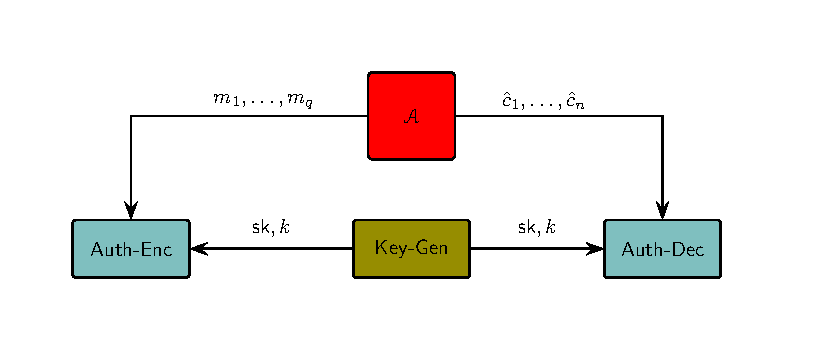
\includegraphics{figures/0604-oracle-interface}
\end{center}

As our aim is to concert the NM-CPA adversary $\AD$ to an IND-CPA adversary $\ADB$, we must be able to perform the decryption operation inside $\ADB$ without an access to the decryption oracle. At first glance, it seems an impossible task. Fortunately, the task is easy when the ciphertext $c_i$ is legitimate ciphertext that was obtained by $\AD$ as a reply to an encryption quary $m_j$. Then we know that $\DEC(c_i)=m_j$.

We will exploit this fact by constructing an interface that stores all encryption queries and corresponding replies as a database, which is later used for mimicking replies for the decryption calls. The schematics of this construction is illustrated below. First, the key of the message authentication code is set up by picking $k\gets\KSPACE$. After that $\ADB$ can simulate $\AENC_{\SK,k}(m_i)$ oracle calls by computing the authentication tag $t_i\gets h(m_i,k)$ and submitting the pair $(m_i,t_i)$ to the encryption oracle $\ENC_\SK(\cdot)$. Let $c_i$ be the corresponding reply. Then the triple $(m_i,t_i,c_i)$ is stored in the encryption table. To decrypt $\hat{c}_1,\ldots\hat{c}_n$, the adversary $\ADB$ uses the encryption table. For each $\hat{c}_i$, it tries to find matching $c_j$ in the table and then use $m_j$ as the decryption $\hat{m}_i$. If some $\hat{c}_i$ is missing form the table, the $\ADB$ halts with zero. Otherwise $\ADB$ returns the value of $\pi(m,\hat{m}_1,\ldots,\hat{m}_n)$

\begin{center}
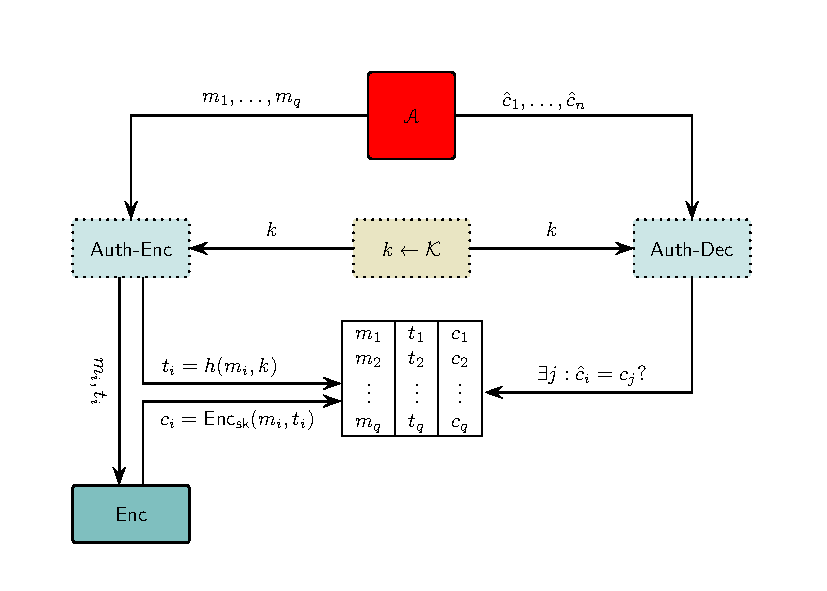
\includegraphics{figures/0604-decryption-simulator}
\end{center}

Let $\LENC$ denote the  event that  $\hat{c}_1,\ldots\hat{c}_n$ are all generated by querying the $\AENC_{\SK,k}(\cdot)$ oracle. Then the event $\neg\LENC$ does not automatically mean that the abrupt halt by $\ADB$ is different from the actual evaluation of the predicate $\pi$ in the non-malleability games. In those games, the game is also halted if the decryption of $\hat{c}_1,\ldots,\hat{c}_n$ fails. More precisely, let $\GDEC$ denote the event that $\AD$ produces a decipherable vector of ciphertexts $\hat{c}_1,\ldots\hat{c}_n$, i.e., $\ADEC_{\SK,k}(\hat{c}_i)\neq \bot$ for all $i\in\set{1,\ldots,n}$. Then
we can decompose the success probabilities as follows:
\begin{align*}
\pr{\GAME_i^\AD=1}&=\pr{\GAME_i^\AD=1\wedge\LENC}\\
&+
\pr{\GAME_i^\AD=1\wedge\neg\LENC\wedge\neg\GDEC}+
\pr{\GAME_i^\AD=1\wedge\neg\LENC\wedge\GDEC}\enspace.
\end{align*} 
We can similarly decompose the success probabilities of $\ADB$ who plays against IND-CPA games $\BGAME_0$ and $\BGAME_1$:
\begin{align*}
\pr{\BGAME_i^\ADB=1}&=\pr{\BGAME_i^\ADB=1\wedge\LENC}\\
&+
\pr{\BGAME_i^\ADB=1\wedge\neg\LENC\wedge\neg\GDEC}+
\pr{\BGAME_i^\ADB=1\wedge\neg\LENC\wedge\GDEC}\enspace,
\end{align*} 
as the substitution of $\ADB$ leads to the game that is identical except for the last line. That is, events $\LENC$ and $\GDEC$ are well defined in games $\BGAME_0^\ADB$ and $\BGAME_1^\ADB$. By the construction
\begin{align*}
\pr{\GAME_i^\AD=1\wedge\LENC}=\pr{\BGAME_i^\ADB=1\wedge\LENC}
\end{align*} 
as $\ADB$ obtains correct decryption values and thus the execution of the last line is identical. Analogously, 
\begin{align*}
\pr{\GAME_i^\AD=1\wedge\neg\LENC\wedge\neg\GDEC}= 0 =
\pr{\BGAME_i^\ADB=1\wedge\neg\LENC\wedge\neg\GDEC}\enspace, 
\end{align*}
since in both games decryption failure causes the abrupt halting. Finally, we also know that   
\begin{align*}
\pr{\BGAME_0^\ADB=1\wedge\neg\LENC\wedge\GDEC}=\pr{\BGAME_1^\ADB=1\wedge\neg\LENC\wedge\GDEC}\enspace, 
\end{align*}
since $\ADB$ halts abruptly for non-legitimately generated ciphertexts. Consequently,
\begin{align*}
\ADVINDCPA{\CS}{\ADB}&=
\abs{\pr{\BGAME_0^\ADB=1}-\pr{\BGAME_0^\ADB=1}}\\
&=\abs{\pr{\BGAME_0^\ADB=1\wedge\LENC}-\pr{\BGAME_1^\ADB=1\wedge\LENC}}\enspace.
\end{align*}
As for any event $\mathsf{E}$ that is defined and has identical probability in both games 
\begin{align*}
\abs{\pr{\GAME_0^\AD=1\wedge \mathsf{E}}-\pr{\GAME_0^\AD=1\wedge \mathsf{E}}}\leq \pr{\mathsf{E}}
\end{align*}
we get by similar reasoning that  
\begin{align*}
\ADVNMCPA{\CS}{\AD}&=
\abs{\pr{\GAME_0^\AD=1}-\pr{\GAME_0^\AD=1}}\\
&\leq\abs{\pr{\GAME_0^\AD=1\wedge\LENC}-\pr{\GAME_1^\AD=1\wedge\LENC}}
+\pr{\neg\LENC\wedge\GDEC}.
\end{align*}
The latter is equivalent to the inequality  
\begin{align*}
\ADVNMCPA{\CS}{\AD}\leq \ADVINDCPA{\CS}{\ADB} + \pr{\neg\LENC\wedge\GDEC} 
\enspace.
\end{align*}

To complete the proof, we need to asses the second term. Note that if the adversary $\AD$ can creates a decipherable vector $\hat{c}_1,\ldots, \hat{c}_n$ without computing all ciphertexts legitimately, then there must exist $\hat{c}_i$ for which the authentication tag $t_i$ was not not computed by the encryption oracle. This leads to new adversary construction $\ADC$ that simulates $\GAME_0$ to the $\AD$ in order to get valid MAC forgery.

\begin{center}
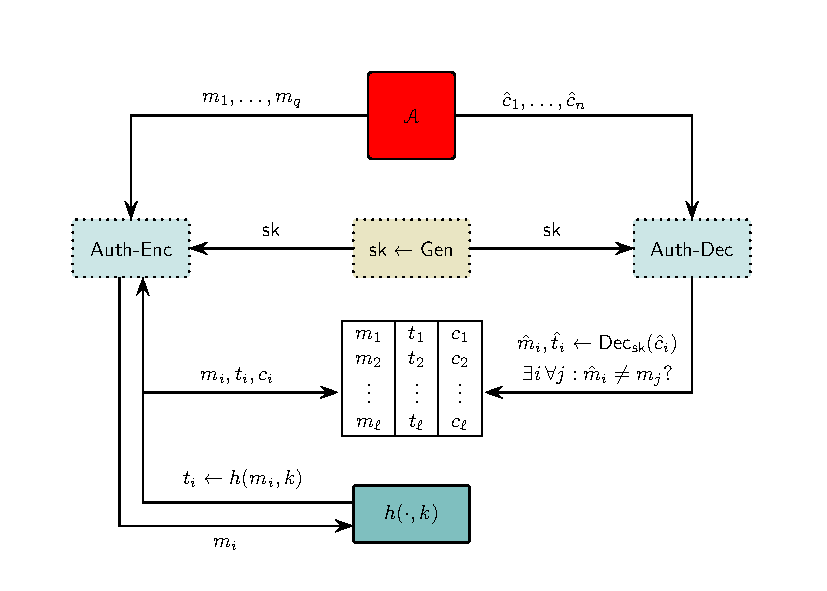
\includegraphics{figures/0604-decryption-simulator-for-mac}
\end{center}

In this construction, the secret key $\SK$ is generated by $\ADC$ who simulates encryption and decryption queries for the $\AD$. For that, $\ADC$ must occasionally query hash values from the hash oracle $h(\cdot,k)$ present in the security game defining security of message authentication codes. The adversary $\ADC$ runs the execution until $\AD$ finishes. After that $\ADC$ decrypts all ciphertexts $\hat{c}_1,\ldots,\hat{c}_n$ and halts if the event $\LENC$ occurs. Otherwise, there must exist $i$ such that $\hat{m}_i$ is not queried form the hashing oracle $h(\cdot,k)$. The pair $\hat{m}_i,\hat{t}_i$ will be the output of $\ADC$. It is easy to see that if the event $\GDEC$ occurs then $\hat{t}_i=h(\hat{m}_i,k)$ and thus $\ADC$ wins the MAC game. Consequently, we have proven that 
\begin{align*}
\pr{\neg\LENC\wedge\GDEC} \leq \ADVMAC{h}{\ADC}\enspace.
\end{align*}   
Careful analysis shows that the overhead in the constructions is $\Theta(q\log q +n\log q)$. Thus for sufficiently small running time of $\AD$ both constructions run in $t$-time and thus $(t,\varepsilon_1)$-IND-CPA security and $(t,\varepsilon_2)$-security of the message authentication code $h$ assures that 
\begin{align*}
\ADVNMCPA{\CS}{\AD}\leq \ADVINDCPA{\CS}{\ADB} + \ADVMAC{h}{\ADC}\leq \varepsilon_1+\varepsilon_2\enspace.
\end{align*}
\end{solution}
\end{document}